The shape of the offering formula is always the same. It opens with the same standard phrase, invokes a god to pass along the offering, lists the offerings then names the recipient.

\section*{\indexed{Htp-di-nsw}}
\addcontentsline{toc}{section}{Htp-di-nsw}

\begin{figure} [H]
	\centering
	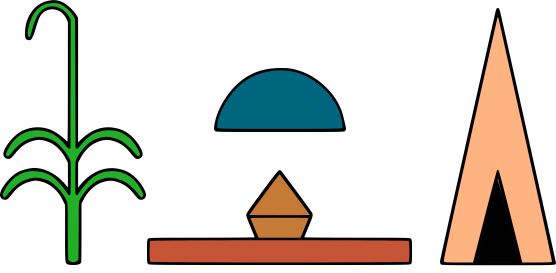
\includegraphics[width=0.4\textwidth]{../images/htp-di-nsw}
	\caption{Htp-di-nsw as commonly rendered in hieroglyphs}
\end{figure}

Many renditions of the offering formula begin with this compound expression. The exact interpretation is debated, but this is often rendered as "a royal offering" or "an offering given by the king".

This expression is sometimes used to describe an offering formula.

By convention the t from \indexed{nswt} is dropped, although it often appears in writing and inscriptions.

The order of the words when written is a case of \textit{\indexed{honorific transposition}}, with the \indexed{nswt} part written first. This is to show the importance of the king, and also applies to names of gods and the word nTr which loosely translates to "god".

\subsection*{Htp}
\addcontentsline{toc}{subsection}{Htp}

\begin{figure} [H]
	\centering
	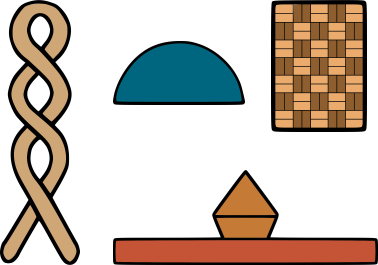
\includegraphics[width=0.275\textwidth]{../images/htp}
	\caption{A more complete spelling of \indexed{Htp} - \textbf{H t p} [Htp]}
\end{figure}

The word \indexed{Htp} has no precise translation into English, and is variously rendered as "contentment", "peace" or "offering". This is sufficient to grasp its true meaning, since offerings are intended to bring comfort and bliss.

\begin{figure} [H]
	\centering
	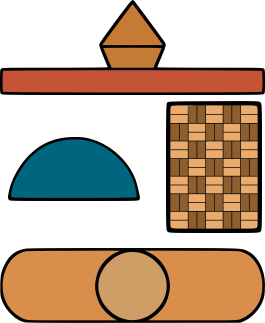
\includegraphics[width=0.175\textwidth]{../images/htp2}
	\caption{Another spelling of \indexed{Htp} - \textbf{Htp} t p [X4]}
\end{figure}

\subsection*{di}
\addcontentsline{toc}{subsection}{di}

\begin{figure} [H]
	\centering
	\includegraphics[width=0.125\textwidth]{../recoloured-tuxscribe-hieroglyphs/png/X8}
	\caption{the (r)di hieroglyph}
\end{figure}

This word is a verb, (r)\indexed{di} - to give, which in older writings is sometimes rendered as \indexed{rdi} rather than di. It also appears later in the formula, but with a suffix pronoun, either .f, .s or .sn depending on the god(s) invoked.

\subsection*{nswt}
\addcontentsline{toc}{subsection}{nswt}

The term nswt means the king or ruler. It was treated with great reverence as the embodiment of the institution of statehood, which was unique in its earliest form.

\section*{prt-xrw}
\addcontentsline{toc}{section}{prt-xrw}

\begin{figure} [H]
	\centering
	\includegraphics[width=0.25\textwidth]{../recoloured-tuxscribe-hieroglyphs/png/O3}
	\caption{the prt-xrw hieroglyph}
\end{figure}

The expression \indexed{prt-xrw} is usually translated as "\indexed{voice offering}", although it more directly means "emerging from voice".

The hieroglyph contains the bread and beer signs, but this is by convention, and doesn't necessarily mean that the voice offering includes bread and beer.

\section*{Offering(s)}
\addcontentsline{toc}{section}{Offerings}

Thee is something of a standard list of offerings, which is usually terminated with the expression xt nbt nfrt wabt Anxt nTr im - all the beautiful and pure things on which a god lives.

\subsection*{Bread - t}
\addcontentsline{toc}{subsection}{t}

Bread.

\subsection*{Beer - Hnqt}
\addcontentsline{toc}{subsection}{Hnqt}

Beer.

\subsection*{Oxen - kAw}
\addcontentsline{toc}{subsection}{kAw}

Oxen.

\subsection*{Fowl - Apdw}
\addcontentsline{toc}{subsection}{Apdw}

Fowl.

\subsection*{Alabaster - Ss}
\addcontentsline{toc}{subsection}{Ss}

Alabaster.

\subsection*{Linen - mnxt}
\addcontentsline{toc}{subsection}{mnxt}

Linen.

\section*{God(s)}
\addcontentsline{toc}{section}{God(s)}

\subsection*{Anubis, he sits on his mountain}

\subsection*{Osiris, lord of Abydos}

\subsection*{Hathor, lady of the west}

\section*{n kA n}

The offering formula is directed at the ka of the recipient.

\section*{Putting it all together}